\documentclass[12 pt]{article}
\usepackage{hyperref, fancyhdr, setspace, enumerate, amsmath,
  lastpage, amssymb, algpseudocode}
\usepackage[margin=1 in]{geometry}
\allowdisplaybreaks
%\usepackage[dvipsnames]{xcolor}   %May be necessary if you want to color links
\hypersetup{
	%colorlinks=true, %set true if you want colored links
	linktoc=all,     %set to all if you want both sections and subsections linked
	linkcolor=black,  %choose some color if you want links to stand out
}
\usepackage{graphicx}
\graphicspath{{Images/}}
\author{Julian Lore}
\date{Last updated: \today}
\title{COMP 360: Algorithm Design}
\pagestyle{fancy}
\lhead{COMP 360}
\chead{\leftmark}
\rhead{Julian Lore}
\cfoot{Page \thepage \ of \pageref{LastPage}}
\newcommand{\tab}[1]{\hspace{.2\textwidth}\rlap{#1}}
\begin{document}
	\onehalfspacing
	\maketitle
	Notes from Hatami Hamed's Winter 2018 lectures.
	\tableofcontents
        \section{01/08/18}
        \href{www.cs.mcgill.ca/~hatami}{Course webpage}. Look at it
        for more details on the grading scheme, assignments and more.
        \paragraph{}We are assumed to have some background in the course, so
        today Hatami will be looking over what we should know for this
        course.
            \subsection{Background Knowledge}
                \begin{itemize}
                \item Tree
                \item Graph, $G=(V,E)$ (all questions in assignments and exams
                  will be written formally, so you should know what the
                  letters mean)
                \item DFS, BFS
                \item Basic algorithm techniques: Greedy algorithms, dynamic
                  programming, divide and conquer, recursion
                \item Running time analysis (Big-O notation)
                \item It's important that you should be able to read math,
                  like precise and formal notation. 
                \end{itemize}
                \subsection{Sample Problems}
                You should be able to read and understand these
                problems. The problems are available
                \href{http://cs.mcgill.ca/~hatami/comp360-W2018/files/test.pdf}{here
                } on the course webpage.
                \paragraph{Example 1} $S$ is a set of positive integers.
                \begin{flalign*}
                  A & = \sum_{x\in S} x^2 &
                  \\ B & = \sum_{\substack{x \in S,\\ x^2 \in S}}x
                \end{flalign*}
                Let $S=\{1,2,3,4,5\}$. What are $A$ and $B$?
                \begin{flalign*}
                  A & = 1^2+2^2+4^2+5^2=1+4+9+16+25 = 46 &
                  \\ B & = 1+2 = 3
                \end{flalign*}
                For $B$, the number must be in $S$ and
                its square must also be in $S$.
                \paragraph{Example 2}
                $M$ is an $n \times n$ matrix. $M_{ij}$ denotes $ij$-entry
                of $M$. The total sum of the entries of $M$ is $100$.
                \begin{flalign*}
                  \sum_{i=1}^n \sum_{j\in \{1,\ldots,n\}\setminus\{i\}}\sum_{r=1}^n M_{ir}&=?&
                  \\ & =\sum_{i=1}^n \sum_{r=1}^n (n-1)M_{ir} =(n-1)100
                \end{flalign*}
                Since we are summing the inner entry $n-1$ times (the
                second summation).
                \\
                Binary expansion/representation.
                \paragraph{Example 3}
                How many digits are in the binary expansion of $n$?
                \begin{flalign*}
                  \text{Ex.} n=5 \implies n=\underbrace{101}_{\text{binary}}
                  \\ \lceil \log_{2}n \rceil \text{ is the answer.}
                \end{flalign*}
                \paragraph{Example 4}
                \begin{flalign*}
                  \sum_{n=0}^k 2^n = ? = 2^{k+1}-1
                \end{flalign*}
                In binary, this is $\underbrace{1111\ldots
                  1}_{\text{binary}}$. Note that this is a geometric sum
                and that you should be able to calculate these.
                \paragraph{Example 5}
                $S=(a_1, a_2, \ldots, a_n)$ a sequence of integers. $E$ is
                the set of even numbers in $\{1, \ldots, n\}$.
                \begin{flalign*}
                  A &= \sum_{i\in E}a_i &
                  \\ \hline
                  \intertext{Example:}
                  S & = \{1,\underline{3},2,\underline{5},4\}
                  \\ A & = ? = \sum_{i\in\{2,4\}} a_i = a_2 + a_4 = 3+5 = 8
                \end{flalign*}
                \paragraph{Example 6}
                $G=(V,E)$ an undirected graph. Suppose to every edge $uv$
                a number $C_{uv}$ is assigned. What does the following
                statement mean?
                \begin{flalign*}
                  \exists c \forall u \in v \sum_{uv \in E}c_{uv}=c
                \end{flalign*}
                There exists some number $c$, such that for every vertex
                we choose, the sum of all edges containing this vertex is
                the same for all vertices.
                    \subparagraph{Example}~\\
                    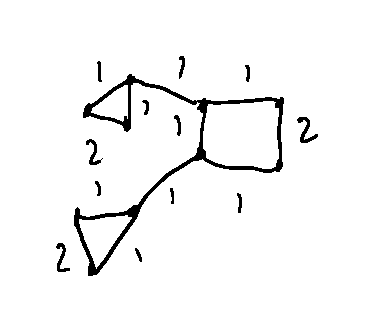
\includegraphics[width=.7\textwidth]{i1.pdf} In this case, $c=3$.
                \paragraph{Example 7}
                $G=(V,E)$ undirected graph degree of every vertex is
                $10$. Suppose to every vertex $v \in V$ a positive integer
                $a_v$ is assigned.
                \\ If $\sum_{v\in V}a_v = 5$ then what is $\sum_{u\in V}
                \sum_{\substack{w\in V:\\ uw\in E}} a_w = ? =\sum_{w \in
                  V}10a_w = 10 \times 5 =50$. Each $a_w$
                appears in the sum $10$ times since the degree of each
                vertex is $10$.
           \subsection{Topics Covered}
                The following are the topics we will be covering in
                this course:
                \begin{itemize}
                \item Network flows (More of like a practice topic for
                  what we'll be seeing in the course, will use the
                  algorithm to solve this problem for seemingly
                  unrelated problems. We'll be doing this a lot in the
                  course, called reduction, where we reduce solving
                  one problem to another problem.)
                \item Linear Programming (Bunch of constraints and
                  want to optimize a linear function). This will be
                  one of the most important concepts we learn in this
                  course.
                \item Midterm
                \item Linear Programming again
                \item NP-Completeness (no good algorithms for problems
                  that seem very basic, useful skill to have even if
                  you aren't a theoretician)
                \item Approximation algorithms (settling for the next
                  best thing for NP-Complete problems, might be able
                  to find an algorithm that approximates things, not
                  exactly optimal, but some sort of factor of how good
                  the approximation is; lots of research happening in
                  this area, better and better approximations). Will
                  use a lot of linear programming here.
                \item Randomized algorithms (randomness can actually
                  help us; probability theory/knowledge of random
                  variables may help a little bit here, but this is
                  the last stretch of the course and not very essential)
                \end{itemize}
         \subsection{Network Flows \\ Max Flow Problem}
            Very important, used in things like game theory.
            \underline{Def}: A flow is a \underline{directed} graph
            $G=(V,E)$ such that:
            \begin{enumerate}
            \item Every edge $e$ has a capacity $c_e \geq 0$.
            \item There is a source $s \in V$.
            \item There is a sink $t \in V$ such that $t\neq s$.
            \end{enumerate}
            \paragraph{Example}~\\
                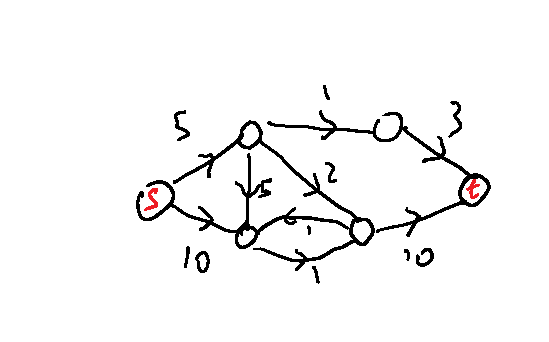
\includegraphics[width=.7\linewidth]{i2.pdf}
            \paragraph{Remark}: For the sake of convenience we make
            the following assumptions.
            \begin{enumerate}
            \item No edge enters the source.
            \item No edge leaves the sink.
            \item All capacities are integers.
            \item There is at least one edge incident to every vertex.
            \end{enumerate}
            \underline{Def}: [flow] A flow is a function $f:E
            \rightarrow \mathbb{R}^+$ such that: (Note that :$\mathbb{R}^+ = \{X \in
            \mathbb{R} | x \geq 0\}$)
            \begin{enumerate}[(i)]
            \item \text{[capacity]} $\forall e \in E, 0 \leq f(e) \leq
              c_e$ (flow cannot be negative nor can it exceed
              capacity)
            \item \text{[conservation]} For every node $u$ other than
              source and sink the amount of flow that goes into $u=$
              the amount of flow that leaves $u$. Formally:
              $$\forall u \in V\setminus\{s,t\} \underbrace{\sum_{vu\in E}f(uv)}_{f^{\text{in}}(u)} = \underbrace{\sum_{uw\in E}f(uw)}_{f^{\text{out}}(u)}$$
            \end{enumerate}
            \paragraph{Example}~\\
                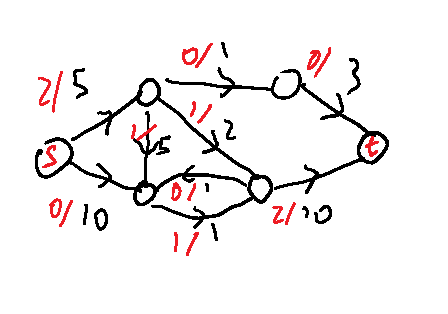
\includegraphics[width=.7\linewidth]{i3.pdf}
            \\ \underline{Def}: $Val(f) = \sum_{su\in E} f(su) =
            f^{\text{out}}(s)$
            \\\noindent\rule{\textwidth}{0.5pt}
            Max Flow Problem: Given a flow network find a flow with
            largest possible value.
    \section{01/10/18}
        \subsection{Max Flow Problem (Continued)}
        Recall: we want to process a flow network, essentially a
        directed graph with a source and a sink.
        \paragraph{A flow network}~\\
        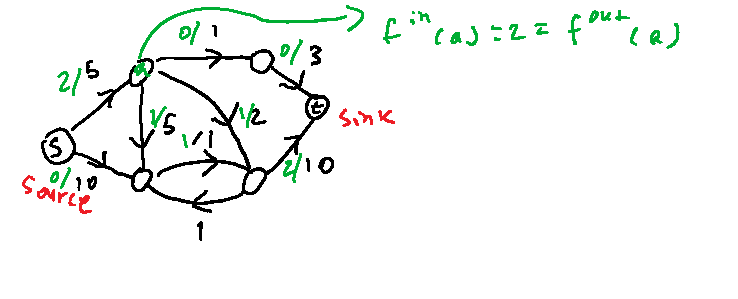
\includegraphics[width=.7\textwidth]{i4.pdf}
        \\ \rule{\textwidth}{0.5pt}
        $val(f)=f^{out}(s)$
        \\ Max Flow Problem: Given a flow network find the maximum
        value of the flow. $2$ is not the optimal value of the
        example. We could change it to:
        \\ 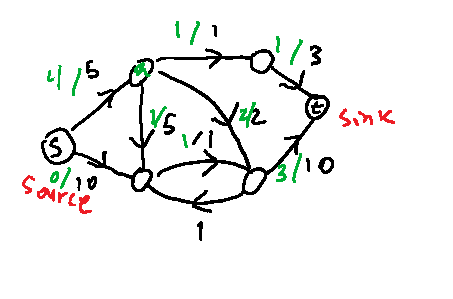
\includegraphics[width=.7\textwidth]{i5.pdf}
        \paragraph{Ford-Fulkerson Algorithm}
        Try to find $s-t$ paths that have not used their capacity and
        push more flow through them. There is a subtlety here
        though, we may run into trouble, like in the following example:
        \\ 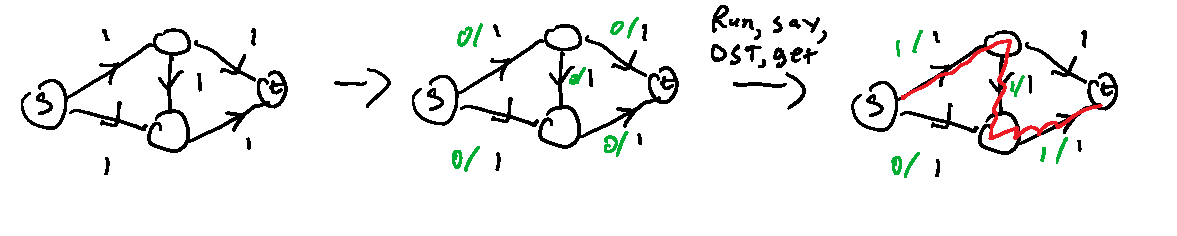
\includegraphics[width=\textwidth]{i6.pdf}
        \\ Now we are stuck. This is \textbf{not optimal}. The
        following is:
        \\ 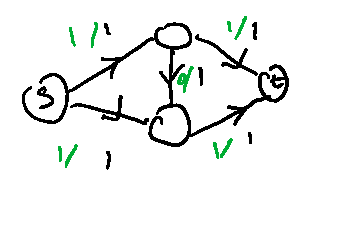
\includegraphics[width=.3\textwidth]{i7.pdf}
        \\ So we must change or else this algorithm won't work. We
        don't want to go back and change the first step, even though
        we are stuck. There is a way that we can change things. Say we
        try to add on more unit of flow:
        \\ 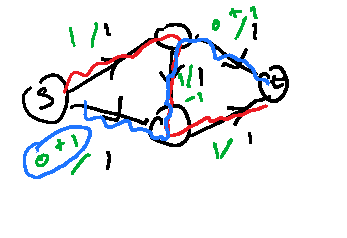
\includegraphics[width=.3\textwidth]{i8.pdf}
        \\ Essentially, the flow we added ``cancels'' the edge in the
        middle and makes it go back. Formally:
        \begin{enumerate}
        \item Start from the all zero flow.
        \item Find a ``path'' (not a real path since we can also
          reverse directions) from $s-t$ such that the edges that are
          in the forward direction have \textbf{unused capacity} (not
          saturated) and the backward edges have \textbf{strictly positive}
          flow on them. Add one unit to forward edges and subtract one
          unit from backwards edges. Repeat this step until we cannot
          find any more paths.
        \end{enumerate}
        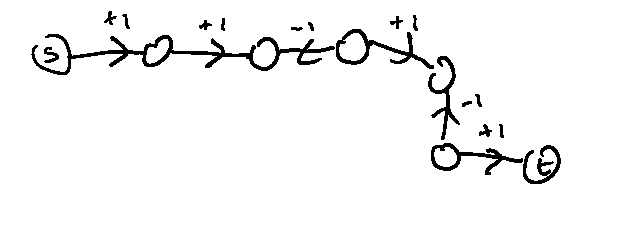
\includegraphics[width=.5\textwidth]{i9.pdf}
        \\ How do we implement this?
        \paragraph{Def} [Residual graph] Given a flow network
        $(G,s,t,\{c_e\})$ and an flow $f$ on $G$, the residual graph
        $G_f$ is as follows (we are already in the middle of the
        algorithm and this graph will tell us which edges are usable):
        \begin{enumerate}
        \item Nodes are the same as $G$.
        \item For every edge $uv \in G$ with $f(uv)<c_{uv}$ (flow
          strictly smaller than capacity), add the edge $uv$ with
          residual capacity $\mathbf{c_{uv}-f(uv)}$ to $G_f$.
        \item For every edge $uv \in G$ with $f(uv)>0$ add the
          opposite edge $\underline{vu}$ with residual capacity $f(uv)$.
        \end{enumerate}
        \rule{\textwidth}{0.5 pt}
        \paragraph{Example} ~ \\
        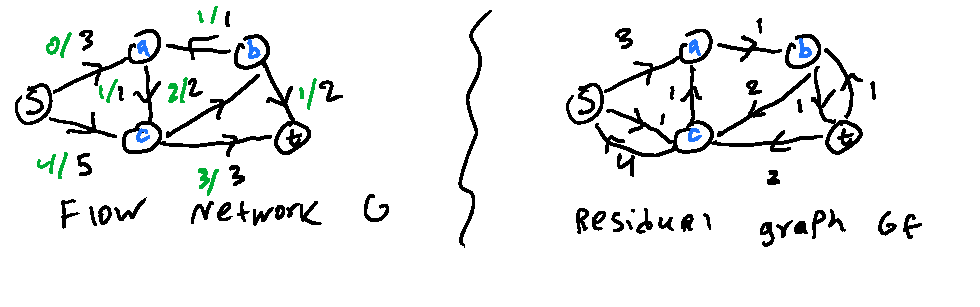
\includegraphics[width=\textwidth]{i10.pdf}
        \\ How do we use the residual graph? Just run a DFS on $G_f$
        to find an $s-t$ path and use it to modify the original flow,
        like so:
        \\ 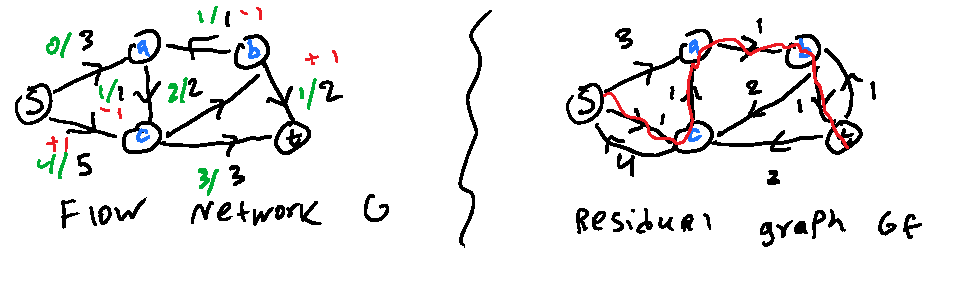
\includegraphics[width=\textwidth]{i11.pdf}
        \paragraph{Pseudocode for Ford-Fulkerson}
        \begin{algorithmic}
          \State Initially set $f(e)=0, \forall e \in E$
          \State Construct $G_f$
          \While{there is an $s-t$-path $P$ in $G_f$}
            \State $f' \gets$Augment$(f,p)$, where Augment means
            increase the flow using path $P$
            \State update $f \gets f'$
            \State update $G_f$
         \EndWhile
        \end{algorithmic}
        How many units of flow can we push if we find the following
        path in $G_f$?
        \\ 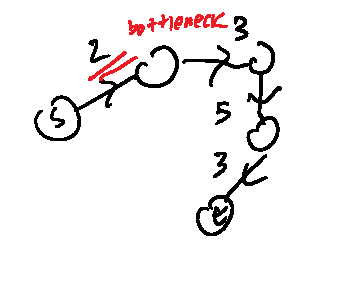
\includegraphics[width=.7\textwidth]{i12.pdf}
        \\ The smallest weight, the bottleneck.
        \begin{algorithmic}
          \State Augment$(f,P)$
          \State Find the bottleneck of $P$, which is the smallest
          residual capacity on $P$.
          \State For forward edges we add this number to their flow.
          \State For backward edges we subtract.
        \end{algorithmic}
        \paragraph{Example}~
        \\ 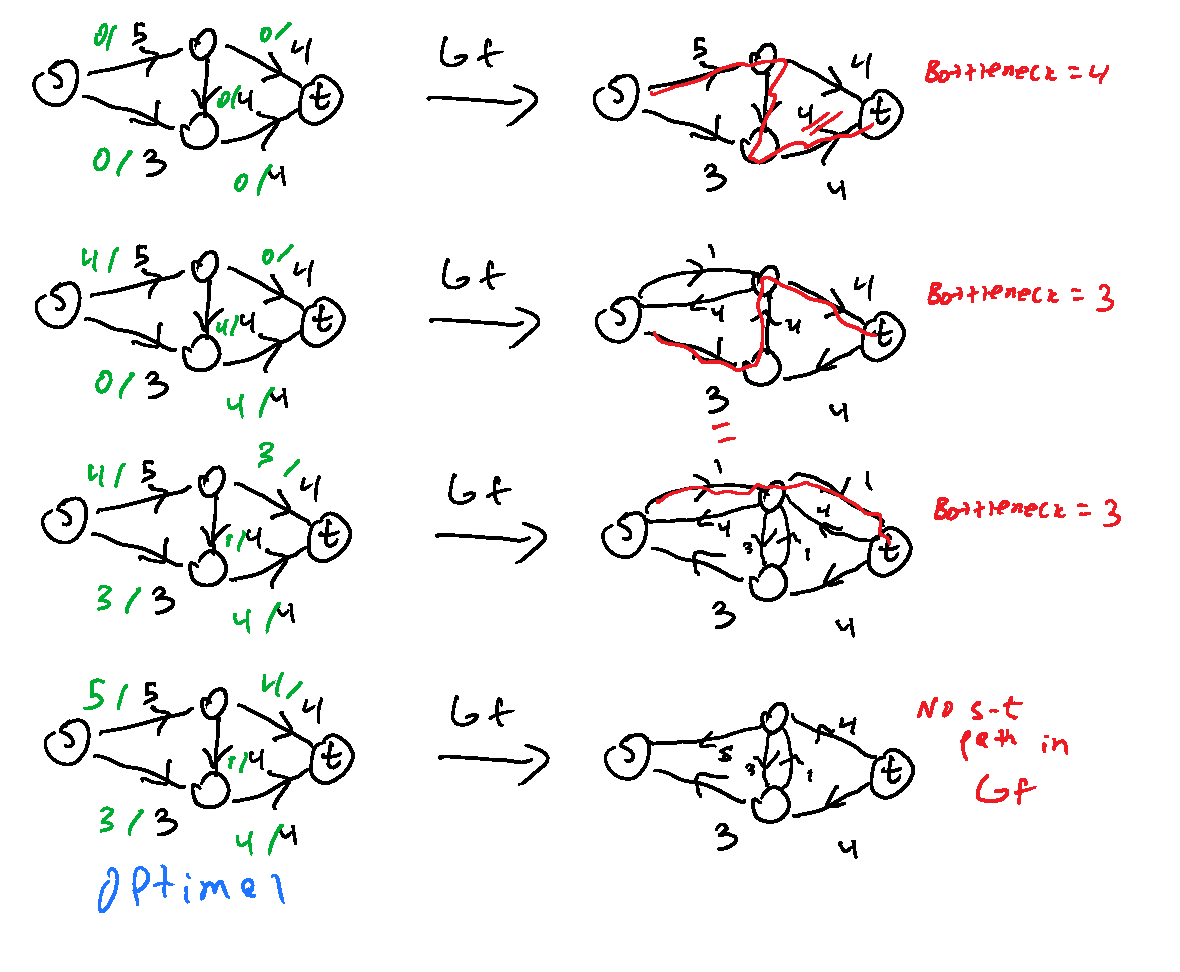
\includegraphics[width=\textwidth]{i13.pdf}
        \paragraph{Claim} FF always returns a valid flow (proof of
        correctness).
        \paragraph{Proof} Residual capacities are chosen so that
        updating with Augment$(f,P)$ will never assign a number to an
        edge that is larger than its capacity or smaller than
        $0$. $\implies$ capacity condition is satisfied throughout the
        algorithm.
        \paragraph{Conservation Condition} $f^{in}(v)=f^{out}(v)$
        \\ 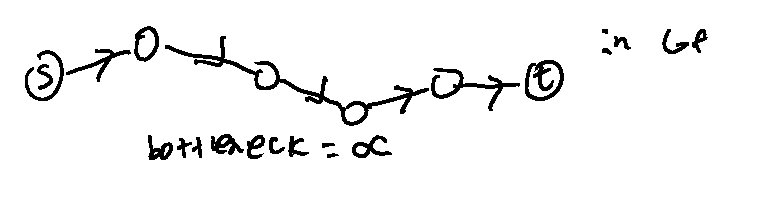
\includegraphics[width=.7\textwidth]{i14.pdf}
        \\ In G:
        \begin{itemize}
        \item Case 1:
        \\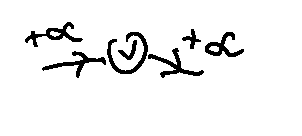
\includegraphics[width=.3\textwidth]{i15.pdf}
          \begin{align*}
            f^{in} \gets f^{in} + \alpha
            \\ f^{out} \gets f^{out} + \alpha
          \end{align*}
          Still the same.
        \item Case 2:
        \\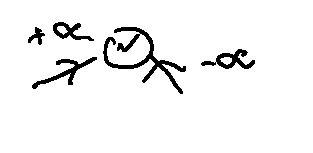
\includegraphics[width=.3\textwidth]{i16.pdf}
          \begin{align*}
            f^{in} \gets f^{in} + \alpha - \alpha
            \\ f^{out} \gets f^{out}
          \end{align*}
          Nothing changed.
        \item Case 3:
        \\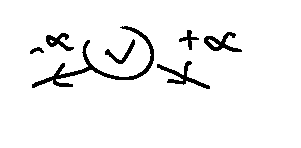
\includegraphics[width=.3\textwidth]{i17.pdf}
          \begin{align*}
            f^{in} \gets f^{in}
            \\ f^{out} \gets f^{out}-\alpha+\alpha
          \end{align*}
          Still equal.
        \item Case 4:
        \\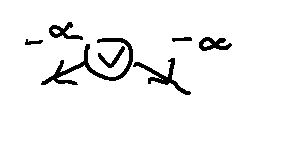
\includegraphics[width=.3\textwidth]{i18.pdf}
          \begin{align*}
            f^{in} \gets f^{in} - \alpha
            \\ f^{out}\gets f^{out} - \alpha
          \end{align*}
          Equal.
        \end{itemize}
        In all cases $f^{in}(v)$ remains equal to $f^{out}(v)$. So we
        have shown that the flow remains valid, but we still don't
        know if it gives us the optimal solution or not.
        \paragraph{Claim} The algorithm terminates.
        \paragraph{Proof} At every iteration, the flow increases by at
        least $1$ unit. It can never exceed the total sum of all the
        capacities, so it has to terminate.
        \paragraph{Running Time} Let $K$ be the largest capacity, $n$
        the number of vertices, $m$ the number of edges. There are at
        most $Km$ iterations. Finding an $s-t$-path:
        $O(m+n)$ (each iteration requires a DFS in the residual graph
        and an update). Augmenting: $(n)$.
        \\ Since we assumed every vertex is adjacent to at least one
        edge $\frac{n}{2}\leq m$ (with this assumption we can just
        talk about $m$). This makes the DFS $O(m)$.
        \\ The total running time:
        $$O(K \times m \times m) = O(Km^2)$$
        Unfortunately not that great if $K$ is a large number. We'll
        try to improve this a little bit later.
        \rule{\textwidth}{0.5pt}
        \paragraph{Def} A cut ($s-t$-cut) in a flow network is a
        partition $(A,B)$ of the vertices such that $s \in A, t\in B$.
        \paragraph{Def} Capacity of this cut is the sum of the
        capacities and edges going from $A$ to $B$.
        \\ 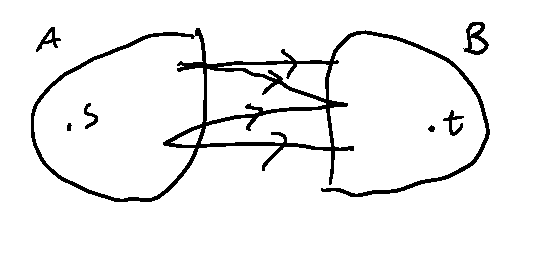
\includegraphics[width=.7\textwidth]{i19.pdf}
        $$cap(A,B)=\sum_{\substack{uv\in E \\ u \in A \\ v \in B}} c_{uv}$$
        \paragraph{Example}
        ~\\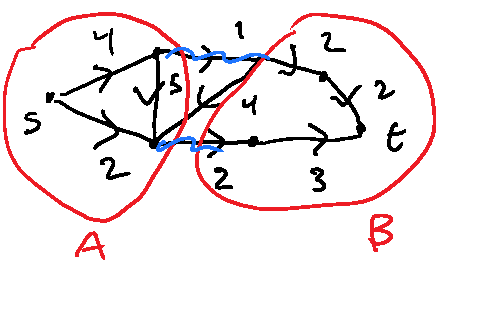
\includegraphics[width=.7\textwidth]{i20.pdf}
        \\ The capacity here is $3$. We see that we can't pass more
        weight from $A$ to $B$, i.e. cuts intuitively tell us
        something about the max flow.
        \\ How many cuts are in this network?
        \\ 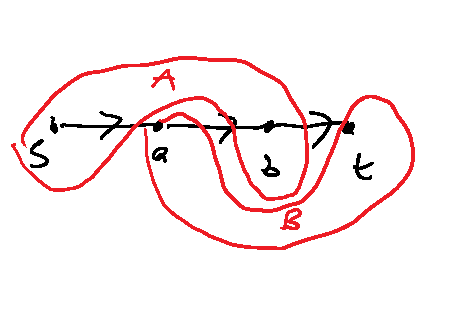
\includegraphics[width=.7\textwidth]{i21.pdf}
        \\ $4$. There's no geometry in cuts, the only restriction is
        that $s$ is in $A$ and $t$ is in $B$, doesn't matter how
        network is drawn.
        \\ A network with $n$ vertices has $2^{n-2}$
        $(s,t)$-cuts. ($n-2$ vertices each with two choices: $2\times
        2 \times \ldots \times 2=2^{n-2}$)
    \section{01/15/18}
        \paragraph{Recall} \textbf{Cut:} Partition of the vertices
        into two parts $A,B$ such that $s\in A, t \in B$.
        \\ 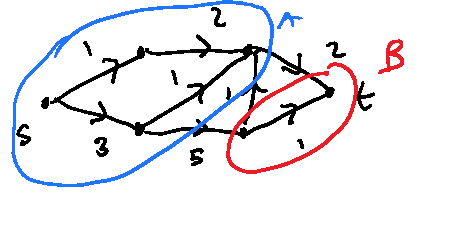
\includegraphics[width=.7\textwidth]{i22.pdf}
        In this example, the capacity is $5+2$
        $$Cap(A,B) = \sum_{\substack{uv \in E \\ u \in A \\ v \in B}}
        C_{uv}$$
        These capacities give us an upper bound on the maximum flow,
        but we have to prove this, intuition isn't enough. So how do
        we prove this?
        \\ \rule{\textwidth}{0.5 pt}
        \paragraph{Recall} For a flow $f:E \to \mathbb{R}^+$,
        $$val(f) = \sum_{su\in E} f(su)$$
        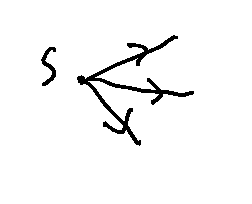
\includegraphics[width=.7\textwidth]{i23.pdf}
        Why do we define it this way? Why not talk about the flow
        going into the sink?
        \\ 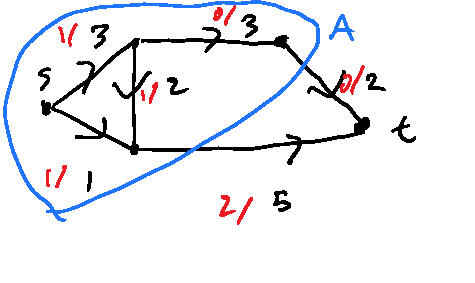
\includegraphics[width=.7\textwidth]{i24.pdf}
        In this example we see that $val=1+1=2$. We can also define a
        flow going into $t$. In this case it would also be $2$. Are
        they equal? Our intuition says yes, because none of the
        intermediate nodes are adding or absorbing flow.
        \\ \rule{\textwidth}{0.5pt}
        \paragraph{Claim} For any $s-t$-cut $(A,B)$, 
        $$val(f) = f^{out}(A) - f^{in}A = \sum_{\substack{uv \in E\\ u
            \in A \\ v \in B}} - \sum_{\substack{uv \in E \\ u \in B
            \\ v \in A}} f(uv)$$
        In the example above, $f^{out}(A) = 1+1+0, f^{in}(A)=0$.
        \\ 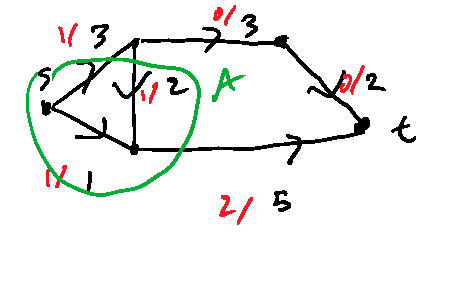
\includegraphics[width=.7\textwidth]{i25.pdf}
        $f^{out}(A)=1+2, f^{in}(A)=1$
        \begin{flalign*}
          val(f)&=\sum_{su\in E}f(su)=f^{out}(s) &
          \\ val(f) & = \sum_{u \in A}f^{out}(u)-f^{in}(u)
        \end{flalign*}
        $f^{out}-f^{in}$ is always $0$, unless $u$ is $s$ or $t$, but
        $t\notin A$.
        \begin{flalign*}
          \sum_{u \in A} \left( \left(\sum_{uv \in E}f(uw)\right) - \left(\sum_{vu \in E}f(vu)\right) \right)
        \end{flalign*}
        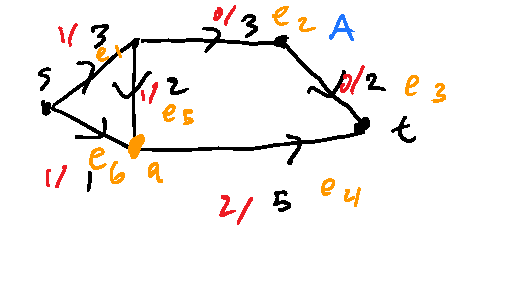
\includegraphics[width=.7\textwidth]{i26.pdf}
        \begin{flalign*}
          f^{out}(s) & = f(e_1)+f(e_6) &
          \\ f^{in}(s)&=0
          \\ f^{out}(a)&=f(e_4)
          \\ f^{in}(a) &= f(e_6)+f(e_5)
          \\
          \\ \left(f(e_1)+f(e_6) - 0\right) + \left(f(e_4)-f(e_6)-f(e_5)\right) & = \underbrace{f(e_1) + f(e_4)}_{f^{out}(a)}-\underbrace{f(e_5)}_{f^{in}(a)}
        \end{flalign*}
        Why did this come out to $f^{out}-f^{in}$? 
        \\ Looking back at the double sum above: If $e$ is an edge
        with both endpoints in $B \implies f(e)$ is not in the sum
        (since each term has at least one vertex in $A$). What if $e$
        has both endpoints in $A$? It will appear in the positive and
        negative sums, so they will cancel out, just like $e_6$ in our
        example.
        \paragraph{Observations}~
        \\ 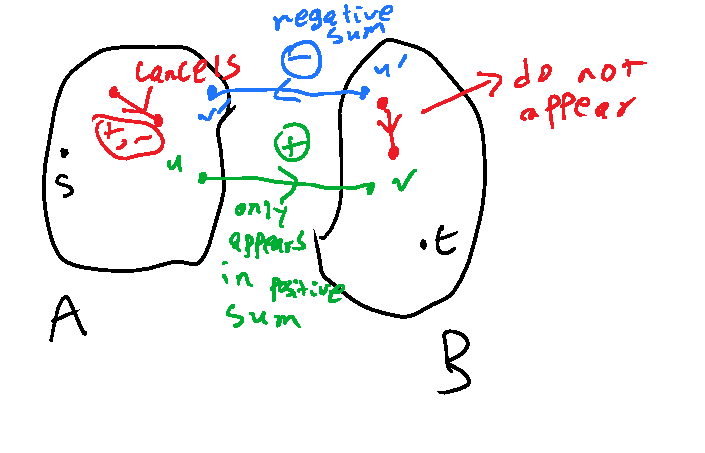
\includegraphics[width=.7\textwidth]{i27.pdf} Because of
        some cancellations here, we can simplify the sum:
        \begin{flalign*}
          \sum_{u \in A} \left(\sum_{uw \in E}f(uw) - \sum_{vu \in E}f(vu)\right)
          \\ = \sum_{\substack{uv \in E \\ u \in A \\ v \in B}}f(uv) - \sum_{\substack{uv \in E\\u \in B \\ v \in A}} f(uv) = f^{out}(A) - f^{in}(A)
        \end{flalign*}
        This concludes the proof of the claim. \hfill $\square$
        \\ Now why does $val(f) = f^{in}(t)$? Take the cut with
        $B=\{t\}$.
        \\ 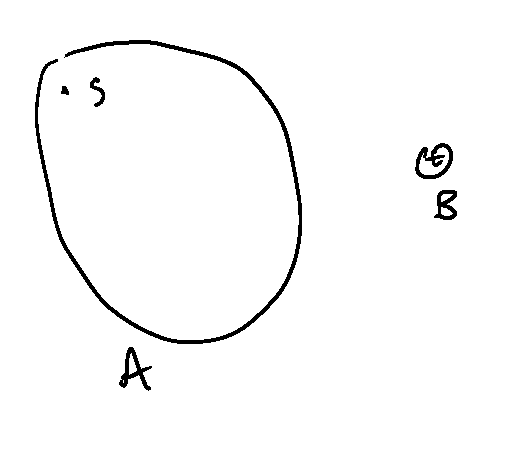
\includegraphics[width=.4\textwidth]{i28.pdf}
        Then by the claim:
        $$val(f) = \underbrace{f^{out}(A)}_{f^{in}(t)} -
        \underbrace{f^{in}(A)}_0$$
        \paragraph{Corollary to this claim} Let $(A,B)$ be a cut, $f$
        be a flow. Then $val(f)\leq cap(A,B)$. i.e. the flow cannot
        exceed the capacity of the cut, any arbitrary cut puts an
        upper bound on the flow. How can we prove this using the
        previous claim?
        \paragraph{Proof}
        \begin{flalign*}
          val(f) & = f^{out}(A) - f^{in}(A) \leq f^{out}(A) = \sum_{\substack{u \in A \\ v \in B \\ uv \in E}}f(uv) \leq \sum_{\substack{u \in A \\ v \in B \\ uv \in E}}C_{uv} = cap(A,B)&
        \end{flalign*}
        In other words, the flow of each edge is bounded by the
        capacity of each edge, but then this is just the definition of
        the capacity of a cut. Now why is this corollary useful? Let's
        look at an example.
        \paragraph{Example} ~
        \\ 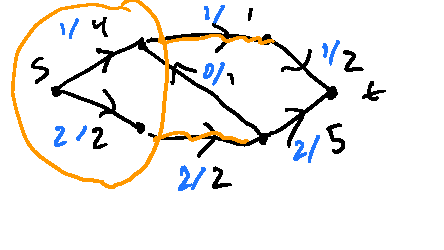
\includegraphics[width = 0.7\textwidth]{i29.pdf}
        $cap(A,B)=1+2 = 3$ and $val=3 \implies$ max flow $= 3$. So if
        we get a flow and are asked if this is the max flow or not,
        either we find a flow with a better value to disprove it, or
        find a cut such that the capacity is the same as the flow, to
        prove that we can't do any better than that.
        \paragraph{Proof of the fact that Ford-Fulkerson finds the max
          flow} Recall:
        \begin{algorithmic}
          \State{FF: start with $f = 0$}
          \While{$s-t$ path $p$ in $G_f$}
            \State{Augment$(f,p)$}
            \State{update $G_f$}
          \EndWhile
        \end{algorithmic}
        Consider the point where Ford-Fulkerson terminates. Let $A^*$
        be the set of the vertices that can be reached from $S$ in
        the residual graph. Why is this a valid cut? Because at
        termination, there are no more $s-t$ paths, so $t \notin A^*$.
        \\ 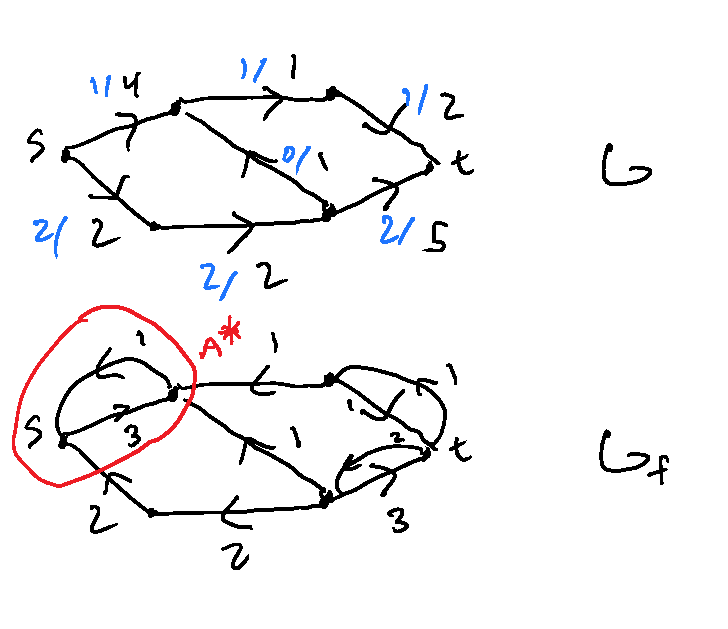
\includegraphics[width=0.7\textwidth]{i30.pdf}
        \\ 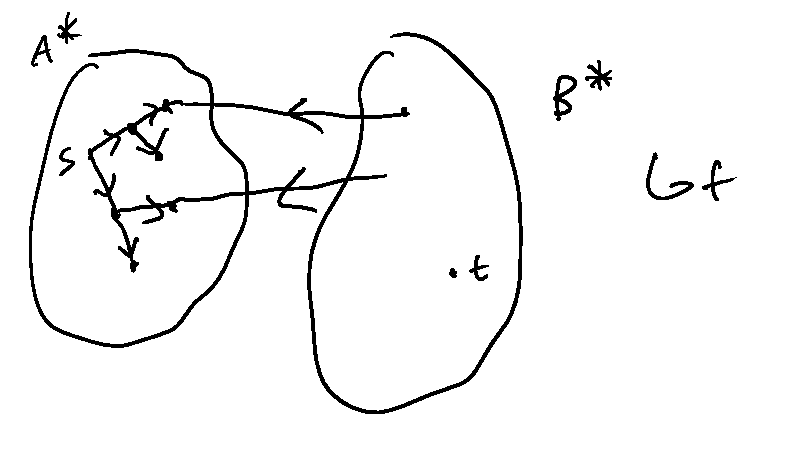
\includegraphics[width=0.7\textwidth]{i31.pdf}
        There are no edges in $G_f$ from $A^*$ to $B^*$, or else the
        endpoint vertex in $B^*$ would be in $A^*$, because $A^*$
        consists of all the vertices we can reach from $s$. Thus:
        if $uv$ is an edge in the original network with $u \in A^*, v
        \in B^*$
        \\ 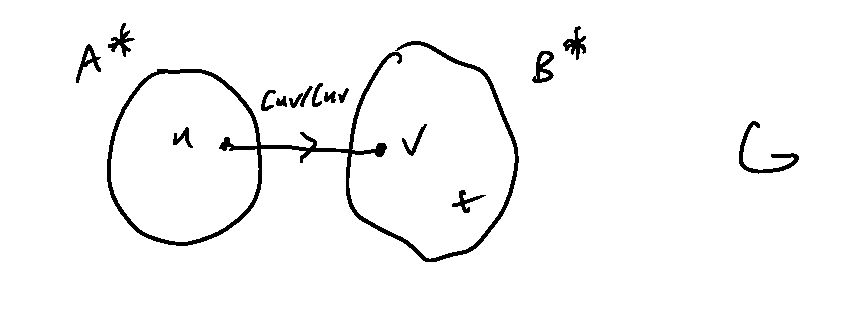
\includegraphics[width=0.7\textwidth]{i32.pdf}
        $f(uv) = C_{uv}$, or else $uv$ edge would be in $G_f$.
        \\ 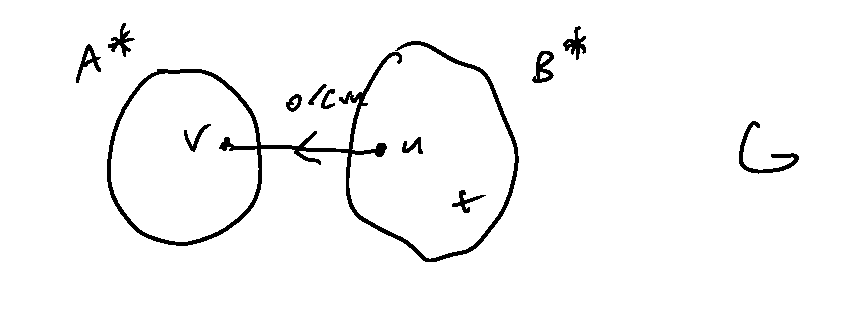
\includegraphics[width=0.7\textwidth]{i33.pdf}
        $f(uv) = 0$, otherwise $vu$ would be in $G_f$.
        Thus:
        \begin{flalign*}
          f^{in}(A^*) & = 0
          \\ f^{out}(A^*) & = \sum_{\substack{u \in A^* \\ v \in B^* \\ uv \in E}} C_{uv} = cap(A^*,B^*)
        \end{flalign*}
        Therefore,
        $$val(f) = f^{out}(A^*)-f^{in}(A^*) = cap(A^*,B^*)$$
        So we showed that Ford-Fulkerson finds the cut that maximizes
        the flow, i.e. Ford-Fulkerson gives us the optimal
        solution. We have:
        \begin{flalign*}
          max-flow \leq cap(A^*,B^*) = val(f) \implies val(f) = max-flow
        \end{flalign*}
        \rule{\textwidth}{0.5pt}
        We showed that Ford-Fulkerson finds max flow. That is, when it
        terminates, $val(f) = max-flow$
        \\ \rule{\textwidth}{0.5pt}
        \paragraph{Problem} Given a flow network how can we find a
        min-cut? Run Ford-Fulkerson and output $(A^*, B^*)$.
        \begin{flalign*}
          \underbrace{val(f)}_{\text{any flow }f} & \leq max-flow \leq min-cut \leq cap(A^*,B^*)
        \end{flalign*}
        When we run Ford-Fulkerson we find $f$ with
        $val(f)=cap(A^*,B^*)$
        $$\implies val(f) = \mathbf{max-flow = min-cut} =
        cap(A^*,B*)$$
        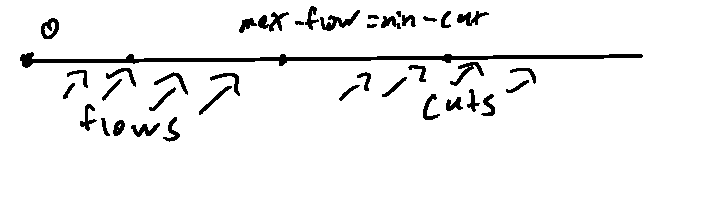
\includegraphics[width=0.7\textwidth]{i34.pdf}
        \paragraph{Thm} For any flow network:
        $$max-flow = min-cut$$
        \section{01/17/18}
        \paragraph{Recall}
        \begin{itemize}
        \item Ford-Fulkerson finds the max flow. 
        \item $Max-flow=Min-cut$. Kind of unexpected/unintuitive that
          they'd be equal. It's pretty intuitive that $min-cut$ is an
          upper bound, but it's surprising that they are equal.
        \item Ford-Fulkerson runs in $O(m^2K)$, where $m$ is the
          number of edges, $K$ is the
          largest capacity of an edge. Can be quite slow if the
          largest capacity is big.
        \item $val(f) =f^{out}(s)=f^{in}(t)=f^{out}(A)-f^{in}(A)$ for
          all cuts $(A,B)$
        \item Ford-Fulkerson can be used to find $min-cut$.
          \\ 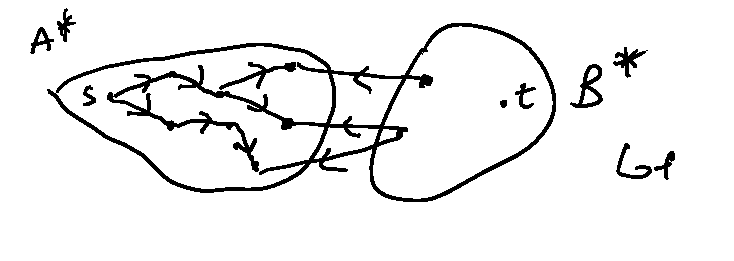
\includegraphics[width=.9\textwidth]{i35.pdf}
          Can't reach $t$ from $s$ at the end of the algorithm in the
          residual graph.
        \end{itemize}
        \paragraph{Question} (Recall all capacities are integers) Is
        it possible to have a $max-flow$ that assigns non-integer
        values to some of the edges? (Remember that the flow function
        is defined as $f:E \to \mathbb{R}^+$) Yes, it is possible:
        \\ 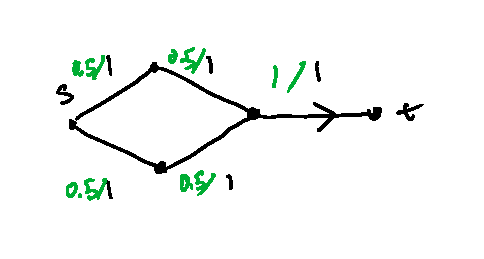
\includegraphics[width=.9\textwidth]{i36.pdf}
        \paragraph{Question} Is there always an all integer
        $max-flow$? Yes because Ford-Fulkerson always outputs integer
        valued flows and we know that it finds $max-flow$. i.e. there
        is at least one all integer $max-flow$, the one that can be
        found by Ford-Fulkerson and we already proved that it gives
        $max-flow$. If you try to prove this directly, it seems very
        hard unless you come up with something like Ford-Fulkerson. So
        we have obtained many important consequences and applications
        from analyzing Ford-Fulkerson.
        \paragraph{Remark} The running time $O(m^2K)$ is not efficient
        when $K$ is a large number. Input size: $\Theta(m \log k)$,
        since we have $m$ edges each that require as much as $\log k$
        bits to write each number between $1-K$. (This is an
        exponential time algorithm)
        \\ 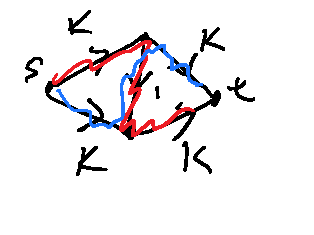
\includegraphics[width=.9\textwidth]{i37.pdf} Running
        Ford-Fulkerson on this graph would require $2^K$ path
        augmentations, alternating between the red and blue path. So
        we want to get rid of this and improve it.
        \subsection{A Faster Ford-Fulkerson}
        \paragraph{Possible Approaches}
        \begin{enumerate}
        \item Always pick the shortest path from $s$ to $t$. This will
          work and leads to an efficient (polytime) algorithm. We will
          not discuss it here. Pretty easy to implement too, just run
          a BFS instead of a DFS.
        \item Try to go with the paths that increase the flow by
          larger numbers. In the above example, we see that the red
          path only increases flow by $1$, instead of the top path
          that can increase it by $K$. This is called the Fattest Path
          approach, where we find an augmenting path with the largest
          bottleneck. However, there is a bit of a problem here,
          finding this path is a bit complicated and not fast. (There
          is a way to implement it by modifying Dijkstra's, but not so
          fast)
          \\ The problem with the first proposed solution is that it
          can't be analyzed easily (although it can be implemented
          easily), whereas the second solution can be analyzed easily
          but not easily implemented.
        \end{enumerate}
        We will do something similar:
        \paragraph{High level description}
        \begin{algorithmic}
          \State Initially set $\Delta = 2^{\lceil \log_2 k \rceil}$,
          that is $\Delta$ is the smallest power of $2$ that is at
          least $K$. (e.g. $K=13 \implies \Delta = 16, K=17 \implies
          \Delta = 32$)
          \While{\underline{there are augmenting paths with
            bottleneck$\geq\Delta$}} use them to augment the flow
          \State When we run out of these we set $\Delta \gets
          \frac{\Delta}{2}$
          \State If $\Delta=1$ here (when we want to decrease it) then stop.
          \EndWhile
        \end{algorithmic}
        How can we check the underlined condition, that there are
        augmenting paths with bottleneck greater than $\Delta$?
        \\ 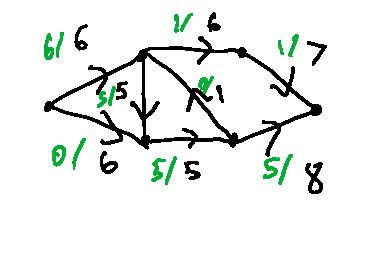
\includegraphics[width=.9\textwidth]{i38.pdf} with
        $\Delta=4$.
        \\In this case, when we build the residual graph we will
        exclude edges that have weight less than $4$. Let
        $G_f(\Delta)$ be the subgraph of $G_f$ consisting only of the
        edges with residual cap $\geq \Delta$. We just need to find an
        $s-t$ path in $G_f(\Delta)$.
        \\ 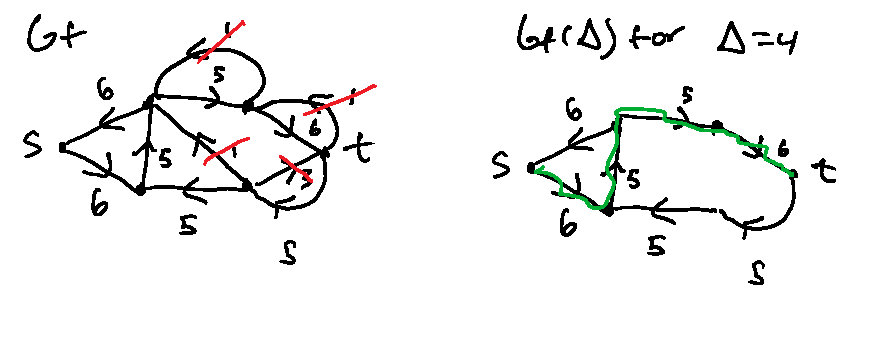
\includegraphics[width=.9\textwidth]{i39.pdf}
        \\ Here bottleneck$\geq \Delta$, we can increase the flow by
        $5$ here.
        \\ We call this scaling.
        \paragraph{Scaling Ford-Fulkerson}
        \begin{algorithmic}
          \State set $\Delta=2^{\lceil \log_2 k \rceil}$, where $K$ is
          the largest capacity.
          \State set $f=0$, construct $G_f$
          \While{$\Delta \geq 1$}
            \While{$\exists$ an $s-t$ path $P$ in $G_F(\Delta)$}
                \State{Augment$(f,p)$}
                \State{update $G_f$}
            \EndWhile
            \State $\Delta \gets \frac{\Delta}{2}$    
          \EndWhile
        \end{algorithmic}
        \paragraph{Running Time}
        \begin{itemize}
        \item Checking if there exists an $s-t$ path: $O(m)$
        \item Augmenting, $O(m)$
        \item Updating $G_f$, $O(m)$
        \end{itemize}
        So we need to understand the number of iterations.
        The other loop has $\lceil \log_@ K \rceil$ iterations. The
        inner loop? (actually will be a bit of work to analyze this.)
        How many times in the $\Delta-phase$?
        \paragraph{Claim} Let $f$
        be the flow at the end of the $\Delta$-phase (when no $s-t$
        paths are in $G_f(\Delta)$). There is a cut $(A,B)$ such
        that $$Max-flow \leq Cap(A,B) \leq val(f)+m\Delta$$
        \paragraph{Proof} Let $A$ be the set of all nodes that can be
        reached from $S$ in $G_f(\Delta)$ (very similar to $min-cuts$
        before)
        \\ 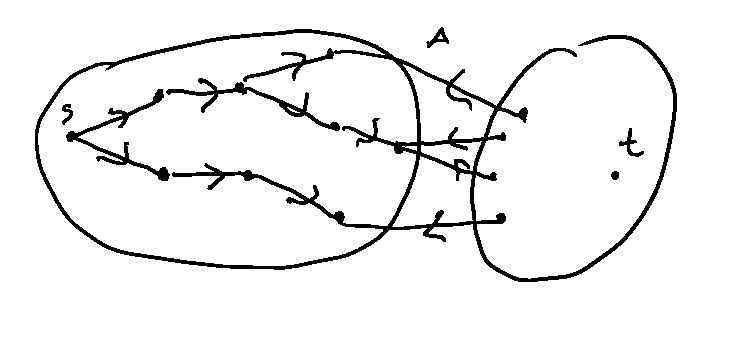
\includegraphics[width=.9\textwidth]{i40.pdf}
        \\ (No edge from $A$ to $B$ in $G_f(\Delta)$, otherwise $A$
        would have been extended further)
        \\ If $e$ is an edge from $A$ to $B$ in the original network:
        \\ 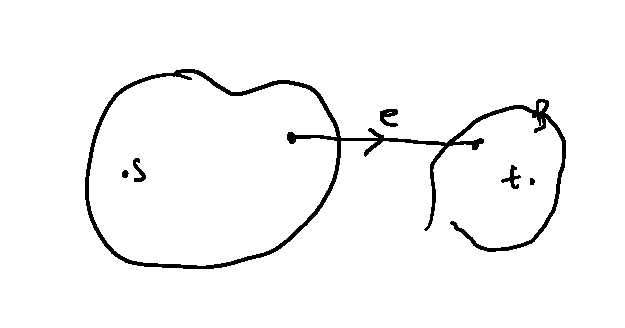
\includegraphics[width=.9\textwidth]{i41.pdf}
        \begin{align*}
          f(e) \geq c_e - \Delta
          \\ c_e - f(e) < \Delta
        \end{align*}
        If $e$ goes from $B$ to $A$:
        \\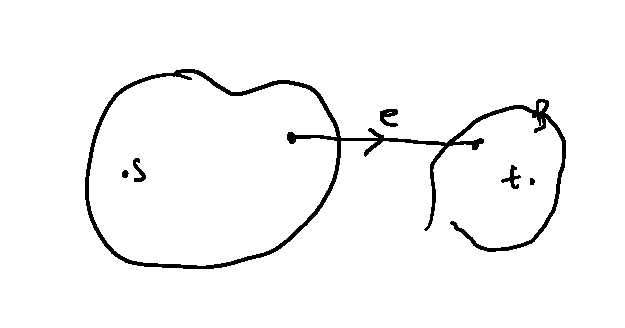
\includegraphics[width=.9\textwidth]{i41.pdf}
        \begin{align*}
          f(e) < \Delta
        \end{align*}
        Or else we could expand $A$.
        \begin{align*}
          val(f) & = f^{out}(A)-f^{in}(A) = \sum_{\substack{e \ from \\ A \ to \ B}} f(e)- \sum_{\substack{e \ from \\ B \ to \ A}}f(e)
          \\ & \geq \sum_{\substack{e \ from \\A \ to \ B}} (c_e - \Delta) - \sum_{\substack{e \ from \\ B \ to \ A}}\Delta = \sum_{\substack{e \ from \\ A \ to \ B}}c_e - \sum_{\substack{e \ from \\ A \ to \ B \\ or \ B \ to \ A}} \Delta
          \\ & = Cap(A,B) -m\Delta \implies val(f) \geq Cap(A,B)-m\delta 
        \end{align*}
        \hfill $\square$
        So we showed $$val(f) \geq Cap(A,B)-m\Delta \geq max-flow -
        m\Delta$$
        Let's look at the flow at the end of the previous phase.
        $$Val(f_{prev})\geq max-flow - 2\Delta m$$ (since we halved
        $\Delta$)
        \\ How many augmentations can we have in the $\Delta$-phase?
        %Every time you increase the $max-flow$, you are increasing it
        %by $\Delta$, and you cannot pass $2\Delta m$, so
        We can have at most $2m$ augmentations in this phase because each one
        increases the value by at least $\Delta$ and starting from
        $max-flow-2m\Delta$ we cannot go above $max-flow$. So the
        number of iterations of this is good as it only depends on
        $m$.
        \\ Back to the analysis, we figured out that the inner loop
        has $\leq 2m$ iterations. So the total running time is:
        \begin{align*}
          O(\log_2 K \times m \times m) = O(m^2 \log K)
        \end{align*}
        Instead of $O(m^2K)$ of the naive Ford-Fulkerson. This is a
        big improvement when $K$ is a huge number.
        \\ One thing is left: Why does this algorithm find the
        $max-flow$? Because when it terminates, $\Delta=1$ and it
        means there are no more augmenting $s-t$ paths in the residual
        graph.
        \paragraph{Remark} This is a special instance of
        Ford-Fulkerson $\implies$ it finds $max-flow$.
      \end{document}
